% !TEX encoding = UTF-8 Unicode
%!TEX root = thesis.tex
% !TEX spellcheck = en-US
\chapter[Result and Discussion]{Result and Discussion}
In this chapter the results of the experiments described in earlier chapters are presented.
The chapter is devided into three sections, covering the 3 different types experiments that were run.
First the experimental optimalization towards our systems properties are presented.
Then the experiment results regarding system performance will be presented.
Finally the results regarding the systems energy efficiency are presented.

\section{Optimization}
Different systems may perform better with different programs.
To ensure that the results we find are represented by programs well suited for the system, the experiments were tested with different degrees of loop unrolling.
By unrolling loop iterations, the task sizes increase.
This reduce the overhead of initiating iterations.
It also reduce overhead related to loop controll, like end of loop tests and dataloading into new memory locations neccessary for each loop iteration.
There is however a limit to how much unrolling can be done.
At some point the size of the task will create difficulties like early cache eviction of data.
The appropriate amount of cache may vary from system to system.
Because of this, experiments were run with different unroll degrees, and on all the processor configurations that will be used for later experiments.

\begin{figure}[H]
  \centering
  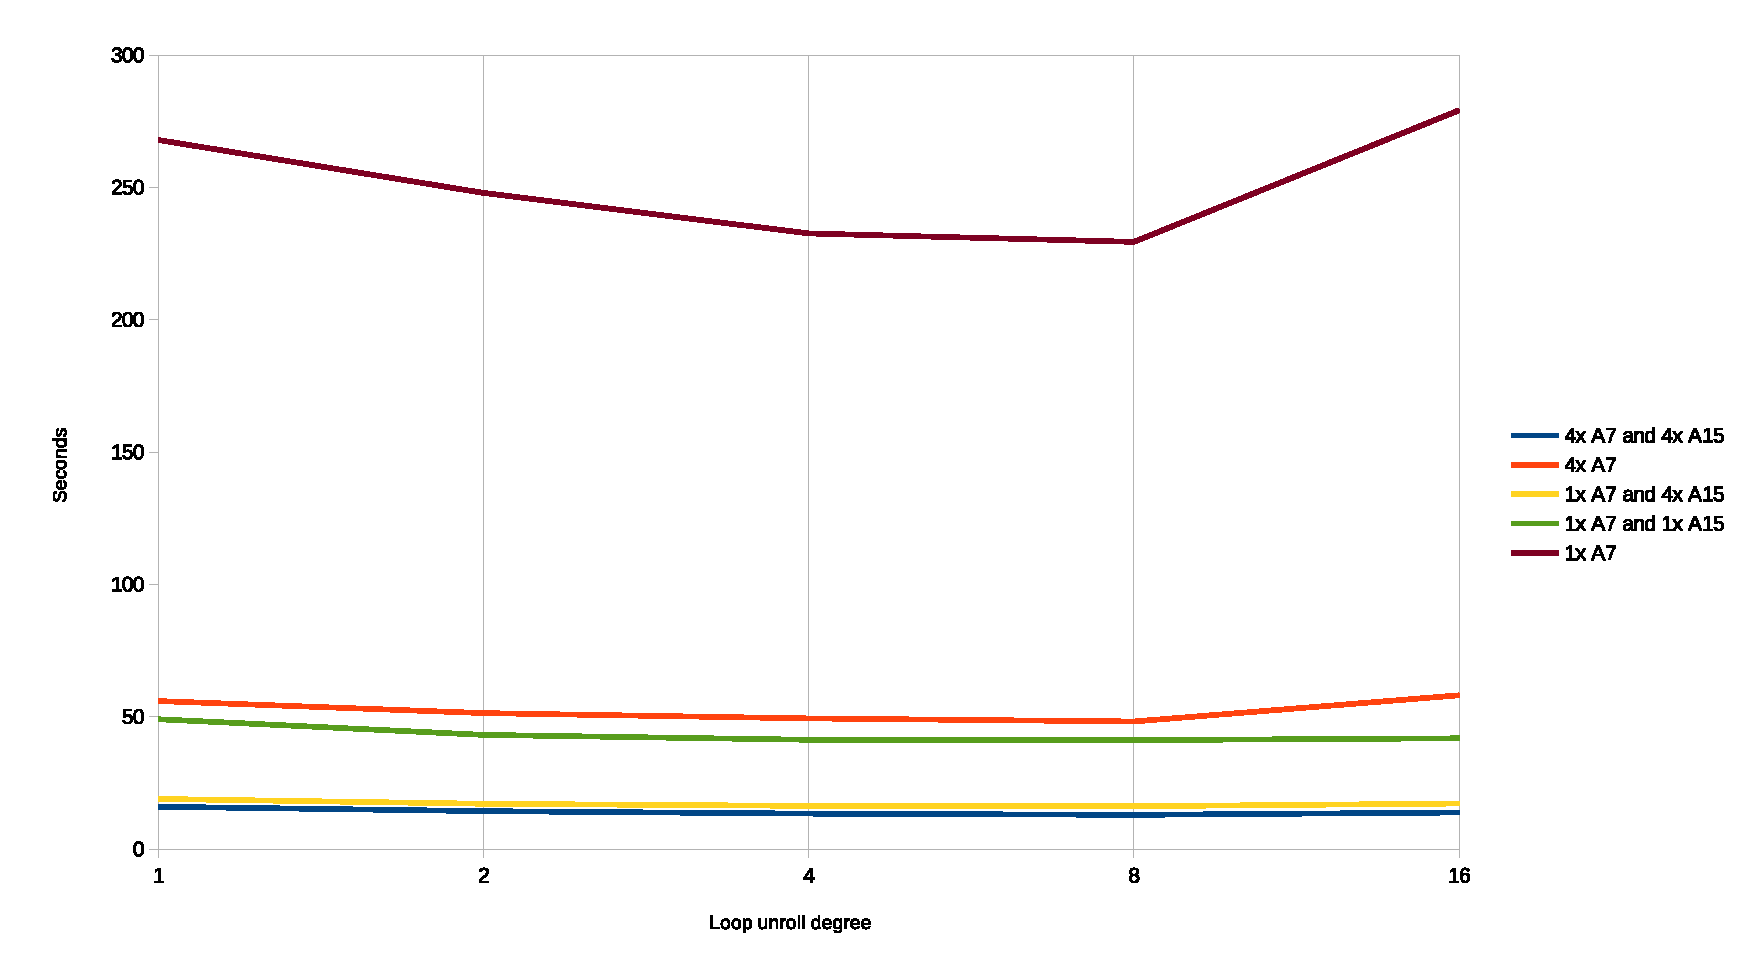
\includegraphics[width=160mm]{fig/loop-unroll-execution-time.eps}
  \caption{Execution time of 2D-Convolution with different degrees of loop unrolling running on different processor configurations. \label{overflow}}
\end{figure}
\begin{table}[H]
  \begin{tabular}{llllll}
    \toprule
    Processor configuration           & \multicolumn{5}{c}{Loop unroll degree} \\
                                      & 1                   & 2         & 4         & 8         & 16 \\
    \midrule
    4x Cortex-A7 and 4x Cortex-A15    & 15.9875             & 14.3006   & 13.3692   & 12.8891   & 13.8013 \\
    4x Cortex-A7                      & 55.8885             & 51.3407   & 49.3267   & 48.1665   & 58.0834 \\
    1x Cortex-A7 and 4x Cortex-A15    & 18.9248             & 17.082    & 16.279    & 16.1658   & 17.1759 \\
    1x Cortex-A7 and 1x Cortex-A15    & 49.0195             & 43.1061   & 41.2549   & 41.1286   & 41.8136 \\
    1x Cortex-A7                      & 267.8882            & 247.8783  & 232.5777  & 229.3884  & 279.1135 \\
    \bottomrule
  \end{tabular}
  \caption{Execution time of 2D-Convolution with different degrees of loop unrolling on different processor configurations. \label{overflow}}
\end{table}

The results show that a loop unroll degree of 8 was optimal for this spesific implementation of 2D-Convolution on ODROID-XU3.
This was observed across the results with all tested processor configurations.
Because of this result, the remainging experiments are all run with a loop unroll degree of 8.

As mentioned loop unrolling is limited.
In 2D-Convolution there are many read write operations in the loop body.
As the size of this loop body increase, the amount of data accessed by each iteration grow.
Eventually this data does no longer fit in cache.
There is reason to suspect that this is what we are observing in the performance loss at loop unroll degree 16.

\section{Performance}
Even with energy efficiency as the focus, performance data are still interesting.
The data are both usefull on their own to observe the power of the system, as well as being a way to compare energy results.
When energy efficiency of a system is measured, it is important to look at the energy data of the system in light of it's computaional power.
A system consuming low amounts of power is not as impressive if it is equally low performing.
These are the results of running 2D-Convolution with 8 as the loop unroll on different processor configurations.

\begin{figure}[H]
  \centering
  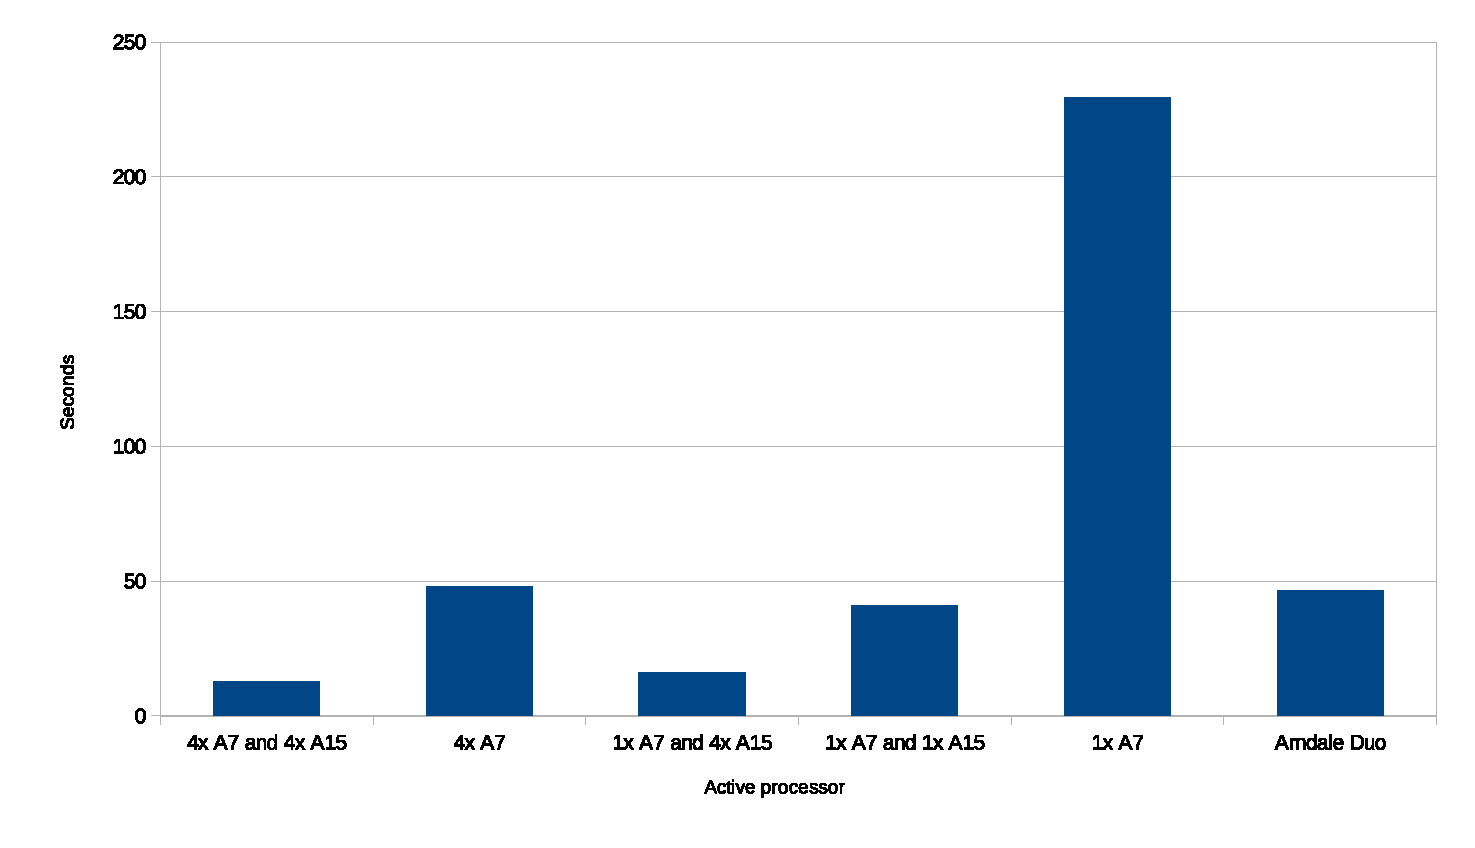
\includegraphics[width=160mm]{fig/execution-time-configurations.eps}
  \caption{Execution time of 2D-Convolution on different processor configurations. \label{overflow}}
\end{figure}

\begin{figure}[H]
  \centering
  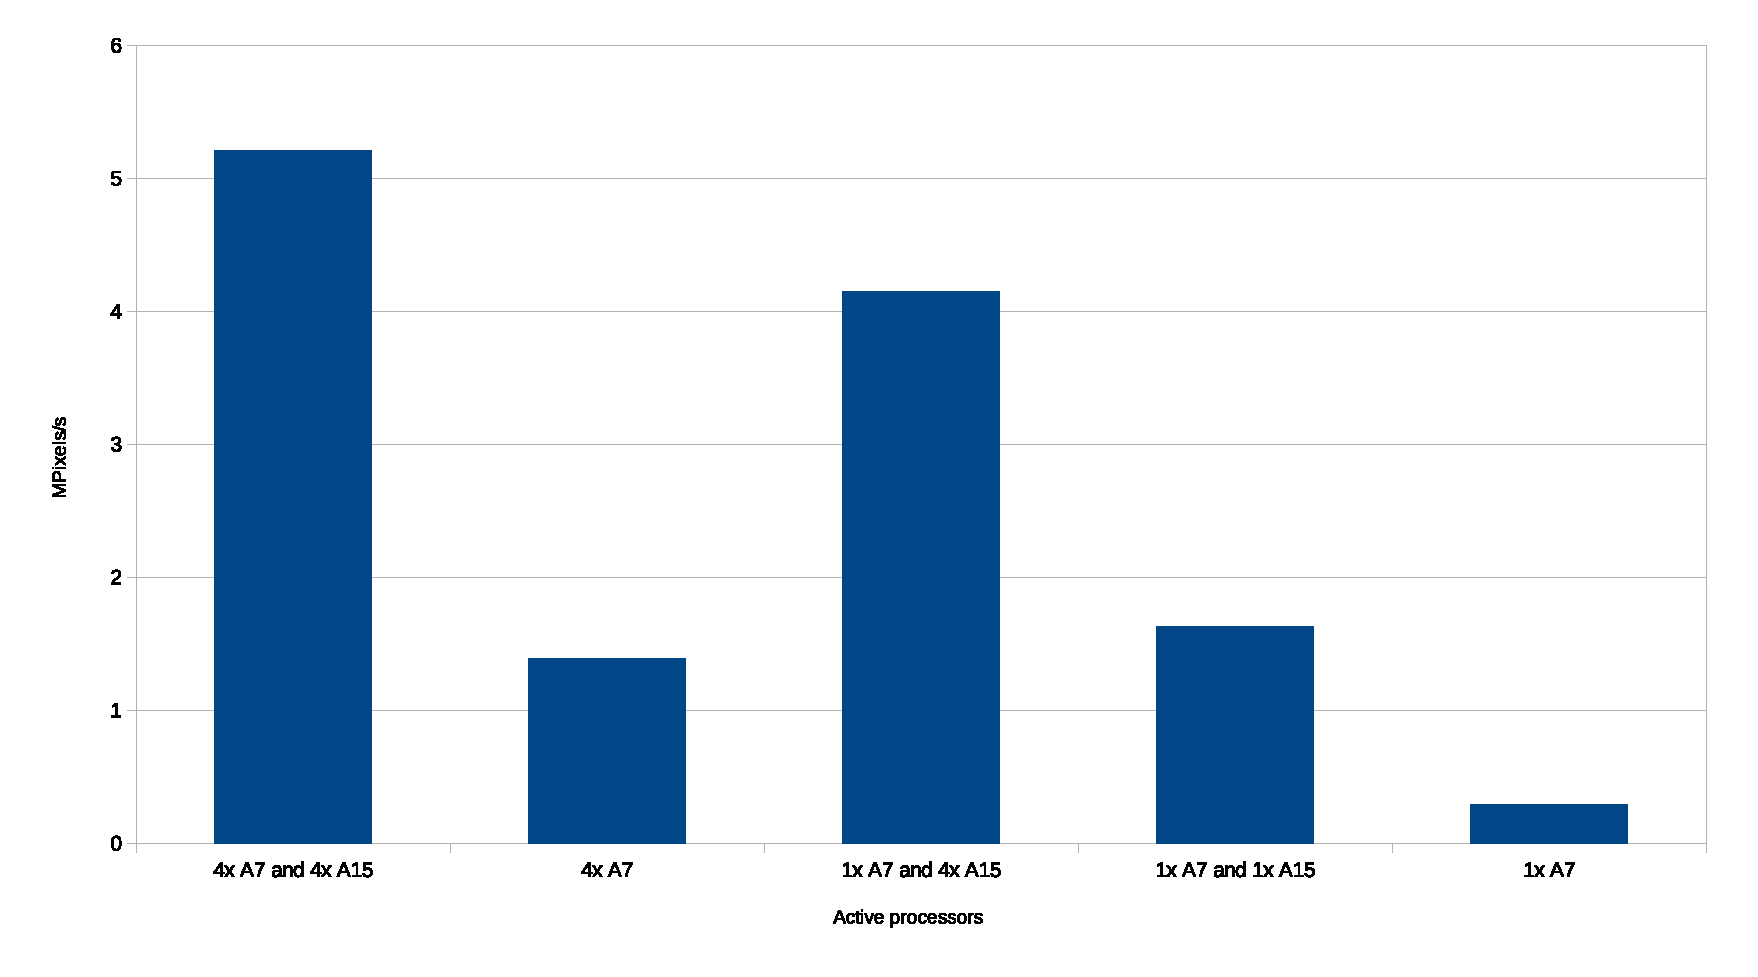
\includegraphics[width=160mm]{fig/mpixelss-configurations.eps}
  \caption{MPixels/s of 2D-Convolution running on different processor configurations. \label{overflow}}
\end{figure}

\begin{table}[H]
  \begin{tabular}{llllll}
    \toprule
    Processor configuration           & Execution time (s)  & Performance (MPixels/s) \\
    \midrule
    4x Cortex-A7 and 4x Cortex-A15    & 12.8891             & 5.2066\\
    4x Cortex-A7                      & 48.1665             & 1.3932\\
    1x Cortex-A7 and 4x Cortex-A15    & 16.1658             & 4.1512\\
    1x Cortex-A7 and 1x Cortex-A15    & 41.1286             & 1.6316\\
    1x Cortex-A7                      & 229.3884            & 0.2925\\
    \bottomrule
  \end{tabular}
  \caption{Performance of 2D-Convolution with different processor configurations. \label{overflow}}
\end{table}


4 x 1 A7 is worse than 1 x 4 A7
4 X 1 stk A7 + 1 stk A15 is better than 4 stk A7 and 4stk A15
All processors perform 3.7 times better than only the small cores.

\section{Energy measurements}
As described in chapter \fullref{setupandmethodology}, seperate energy measurements for the different SoC components were gathered during execution of the experiments.
The each of the 4 components value was logged every 200 ms.
In figure \ref{powerovertime} you can see the raw energy measurements for a single execution of 2D-Convolution running on all 8 processors.
We can here observe the energy consumption of the program throughout the execution for different components.
The total energy consumption can be calculated from the data.
But overvations regarding power uage during different execution stages can also be analysed.
The same kind of data were gathered for a range of different processor configurations.

\begin{figure}[H]
  \centering
  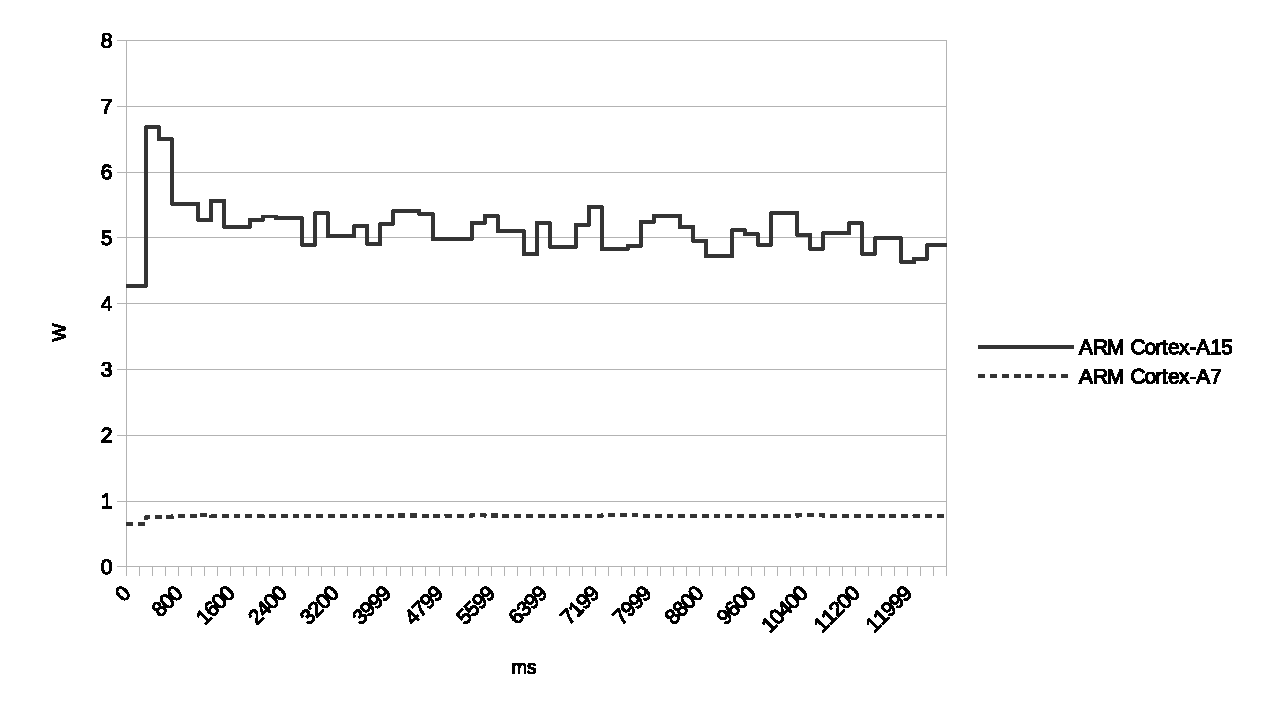
\includegraphics[width=160mm]{fig/power-over-time.eps}
  \caption{Power cunsumption for the large and small cores during executioin of 2D-Convolution with unroll 8x. This is a full execution running on all 8 processors. \label{overflow}}\label{powerovertime}
\end{figure}
There is a spike in power consumption on both the small and large cores at the start of the execution.
This spike can be caused by a lot of different reasons.
There is not enough data to know what caused it.
Typical reasons for such spikes are intense opetaions during initiation of the program, or simply hardware implementations causing a power surge when processor cores are suddenly powered from idle state.
For the rest of the execution there are variations in power consumption, but the consumption vary around the same general level.

\begin{figure}[H]
  \centering
  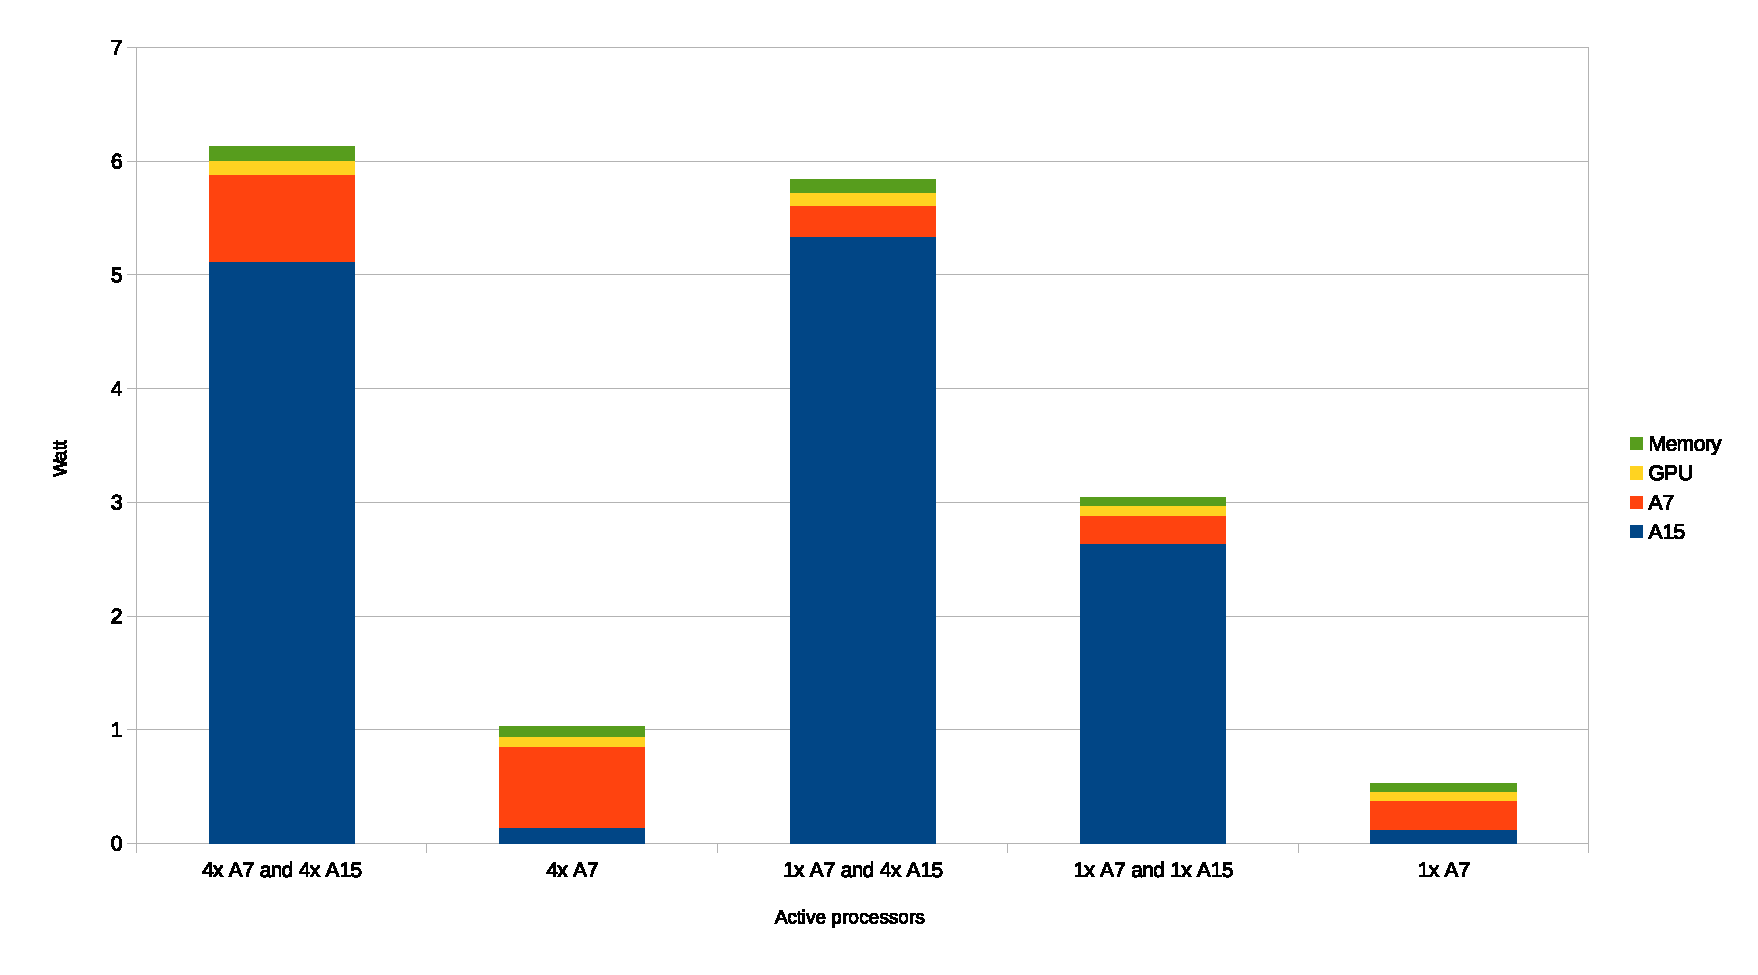
\includegraphics[width=160mm]{fig/power-configurations.eps}
  \caption{Average power consumed per second for different processors configurations running 2D-Convolution. The colors indicate different components, and the full height of each column is the accumulated total for the whole system.\label{overflow}} \label{power-configurations}
\end{figure}

\begin{table}[H]
  \begin{tabular}{llllll}
    \toprule
    Processor configuration         & \multicolumn{5}{c}{Power consumption per second for each component} \\
                                    & Cortex-A15  & Cortex-A7 & Mali-T628 & Memory  & Total \\
    \midrule
    4x Cortex-A7 and 4x Cortex-A15  & 5.1156          & 0.7693        & 0.1206        & 0.1208  & 6.1264 \\
    4x Cortex-A7                    & 0.1362          & 0.7157        & 0.0899        & 0.0817  & 1.0238 \\
    1x Cortex-A7 and 4x Cortex-A15  & 5.3356          & 0.2758        & 0.1161        & 0.1098  & 5.8373 \\
    1x Cortex-A7 and 1x Cortex-A15  & 2.6341          & 0.2540        & 0.0818        & 0.0755  & 3.0456 \\
    1x Cortex-A7                    & 0.1197          & 0.2535        & 0.0813        & 0.0709  & 0.5256 \\
    \bottomrule
  \end{tabular}
  \caption{Execution time of 2D-Convolution with different degrees of loop unrolling on different processor configurations. \label{overflow}}
\end{table}
Using the data gathered for each component in different processor configurations we can examine their efficiency.
These data are presented in figure \ref{power-configurations}.

As expected we see that the power of the ARM Cortex-A7s is a lot lower than the power of the ARM Cortex-A15.
Turning off the power hungry Cortex-A15s reduce the total power to a sixth (0.17).

Turning off 3 Cortex-A15 cores only reduce the power to about half (0.51).
Similarly turning off 3 Cortex-A7 cores only reduce power to a bit more than two thirds (0.35).
Even turning all the Cortex-A15 cores off still leave some power consumed by them.


\begin{figure}[H]
  \centering
  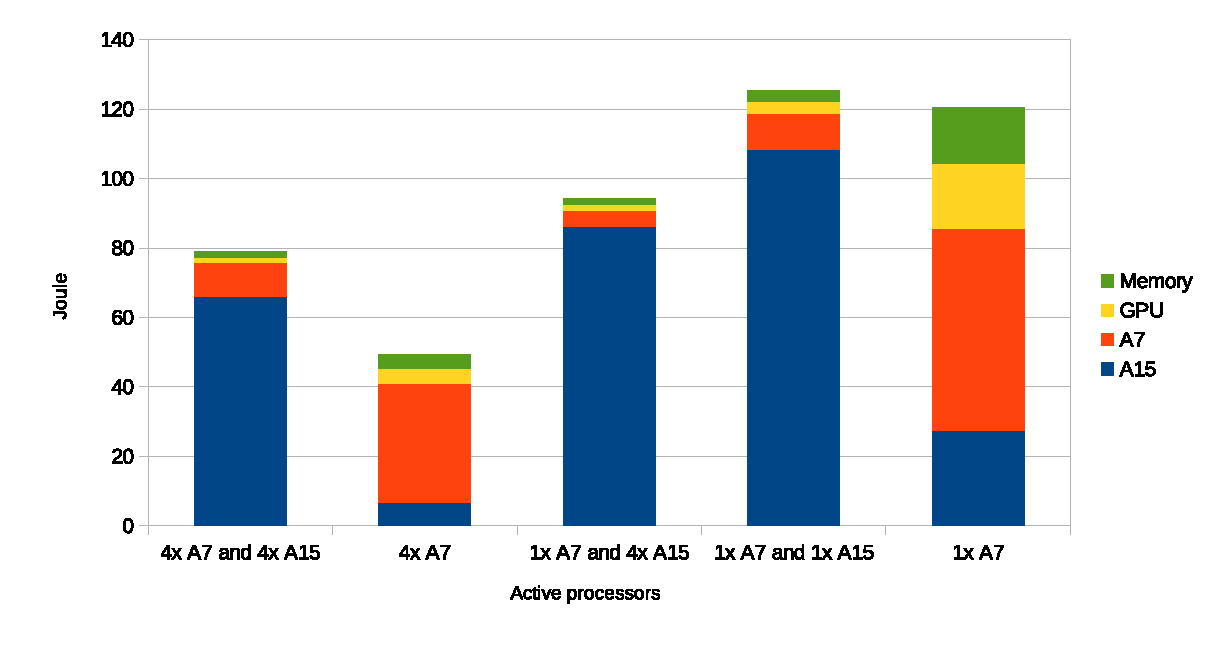
\includegraphics[width=160mm]{fig/power-consumed-configurations.eps}
  \caption{Energy delay product indicating the total amount of power consumed executing the whole 2D-Convolution program. The colors indicate different components, and the full height of each column is the accumulated total for the whole system.\label{overflow}}
\end{figure}

\section{Energy Delay product}

